\section{Documentation du code}

\begin{frame}{Motivation}
\begin{itemize}
\item Une forme de contradiction entre écrire une doc et écrire du code commenté
\item Certains outils proposent de générer la doc à partir du code lui-même
\item Avantages
\begin{itemize}
\item On ne fait qu'une fois le travail
\item Mise à jour de la doc \textit{automatique}
\end{itemize}
\item Inconvénients 
\begin{itemize}
\item Ca ne dispense pas de certaines docs complémentaires
\item Il faut mettre des commentaires (pertinents) dans son code
\end{itemize}
\end{itemize}
\end{frame}

\begin{frame}{Doxygen}
\begin{itemize}
\item Doxygen est un outil de génération de documentation à partir du code et de ses commentaires
\item Multi-langages 
\item Multi-cibles 
\item S'intègre bien à des chaînes de production de code (Makefile...)
\item \url{http://www.doxygen.nl}
\end{itemize}
\end{frame}

\begin{frame}[fragile]
\frametitle{Commentaires}
\begin{itemize}
\item Style C avec deux \texttt{*}
\begin{lstlisting}
/** 
  *   ... documentation 
*/
\end{lstlisting}
\item Style C avec un \texttt{!}
\begin{lstlisting}
/*! 
  *   ... documentation 
*/
\end{lstlisting}
\item Style C++ avec trois \texttt{*}
\begin{lstlisting}
/// 
///   ... documentation 
///
\end{lstlisting}
\item Style C++ avec un \texttt{!}
\begin{lstlisting}
//! 
//!   ... documentation 
//!
\end{lstlisting}
\end{itemize}
\end{frame}

\begin{frame}[fragile]
\frametitle{Entête de fichier}
\begin{lstlisting}
/**
 * \file main.c
 * \brief Programme de tests.
 * \author Franck.H
 * \version 0.1
 * \date 11 septembre 2007
 *
 * Programme de test pour l'objet de gestion des chaines de caracteres Str\_t.
 *
 */
\end{lstlisting}
\end{frame}

\begin{frame}[fragile]
\frametitle{Documentation d'une fonction}
\begin{lstlisting}
/**
 * \fn static Str_t * str_new (const char * sz)
 * \brief Fonction de creation d'une nouvelle instance d'un objet Str_t.
 *
 * \param sz Chaine a stocker dans l'objet Str_t, ne peut etre NULL.
 * \return Instance nouvellement allouee d'un objet de type Str_t ou NULL.
 */
static Str_t * str_new (const char * sz);
\end{lstlisting}
\end{frame}


\begin{frame}[fragile]
\frametitle{Exemple complet en C++ (1/)}
\begin{lstlisting}
#ifndef CPLAYER_H_
#define CPLAYER_H_
 
/*!
 * \file CPlayer.h
 * \brief Lecteur de musique de base
 * \author hiko-seijuro
 * \version 0.1
 */
#include <string>
#include <list>
 
/*! \namespace player
 * 
 * espace de nommage regroupant les outils composants 
 * un lecteur audio
 */
namespace player
{
  /*! \class CPlayer
   * \brief classe representant le lecteur
   *
   *  La classe gere la lecture d'une liste de morceaux
   */
  class CPlayer
  {
  private:
    std::list<string> m_listSongs; /*!< Liste des morceaux*/
    std::list<string>::iterator m_currentSong; /*!< Morceau courant */
\end{lstlisting}
\end{frame}


\begin{frame}[fragile]
\frametitle{Exemple complet en C++ (2/)}
\begin{lstlisting}
  public:
    /*!
     *  \brief Constructeur
     *
     *  Constructeur de la classe CPlayer
     *
     *  \param listSongs : liste initial des morceaux
     */
    CPlayer(std::list<string> listSongs);
 
    /*!
     *  \brief Destructeur
     *
     *  Destructeur de la classe CPlayer
     */
    virtual ~CPlayer();
 
  public:
    /*!
     *  \brief Ajout d'un morceau
     *
     *  Methode qui permet d'ajouter un morceau a liste de
     *  lecture
     *
     *  \param strSong : le morceau a ajouter
     *  \return true si morceau deja present dans la liste,
     *  false sinon
     */
    bool add(std::string strSong);
\end{lstlisting}
\end{frame}


\begin{frame}[fragile]
\frametitle{Exemple complet en C++ (3/3)}
\begin{lstlisting}
    /*!
     *  \brief Morceau suivant
     *
     *  Passage au morceau suivant
     */
    void next();
 
    /*!
     *  \brief Morceau precedent
     *
     *  Passage au morceau precedent
     */
    void previous();
 
    /*!
     *  \brief Lecture 
     *
     *  Lance la lecture de la liste
     */
    void play();
 
    /*!
     *  \brief Arret
     *
     *  Arrete la lecture
     */
    void stop();
  };
};
\end{lstlisting}
\end{frame}

\begin{frame}{Ensuite}
\begin{itemize}
\item Générer un fichier de \textit{template}
\texttt{doxygen -g htmlDox}
\item Editer le fichier de configuration (c'est du texte)
\item Générer la doc proprement dite 
\texttt{doxygen htmlDox}
\item Voir la doc dans le sous-répertoire \texttt{html}
\end{itemize}
\end{frame}

\begin{frame}{Résultat}
\begin{center}
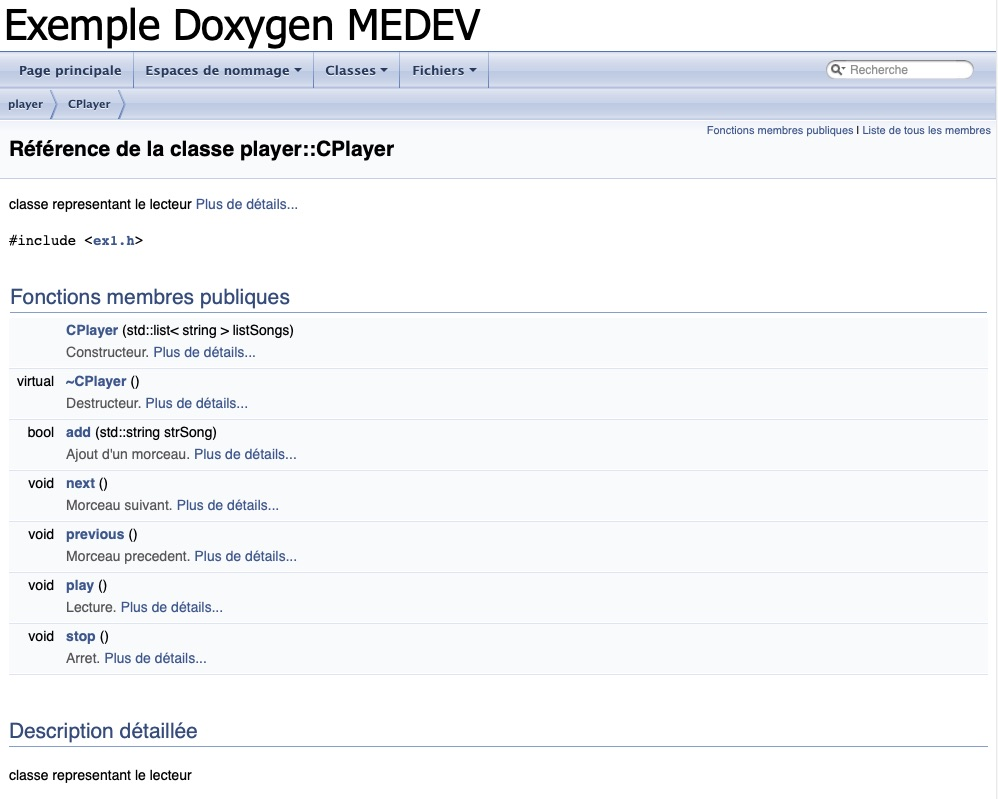
\includegraphics[height=\textheight]{fig/doxygen.jpg}
\end{center}
\end{frame}
